\chapter{HASIL DAN PEMBAHASAN}
\section{Analisis Kapasitas Board FPGA}
....

\section{Hasil Pelatihan Model CNN}
\begin{figure}[H]
	\centering
	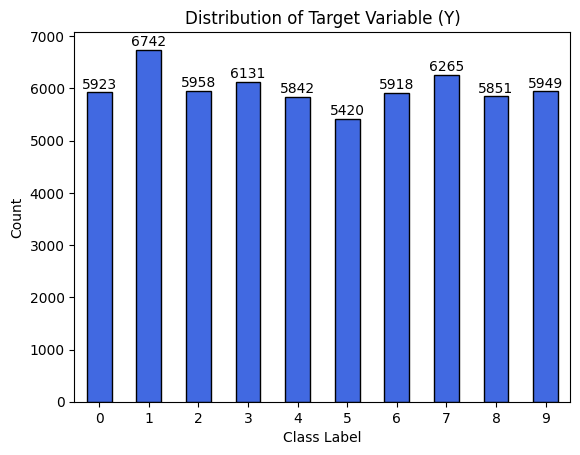
\includegraphics[width=0.95\textwidth]{gambar/data_train_distribution.png}
	\caption{Distribusi \emph{Training Dataset} yang digunakan}
	\label{fig:model-dataset}
\end{figure}

	\subsection{Arsitektur Target Model CNN}
	....
	\begin{figure}[H]
      \centering
      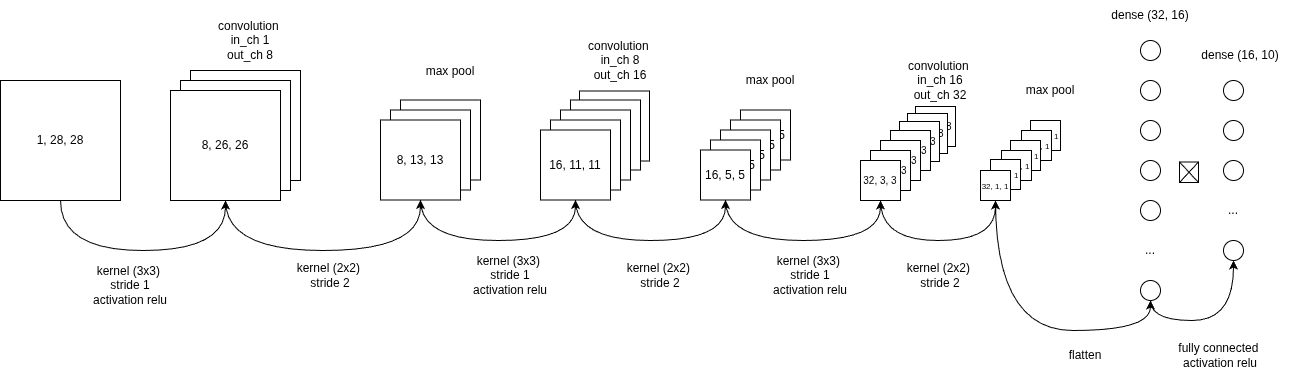
\includegraphics[width=0.95\textwidth]{gambar/cnn architecture.png}
      \caption{Arsitektur Model CNN}
      \label{fig:model-architecture}
  	\end{figure}

	\subsection{\emph{Loss} dan \emph{Akurasi} Hasil Pelatihan}
	....
	\begin{figure}[H]
      \centering
      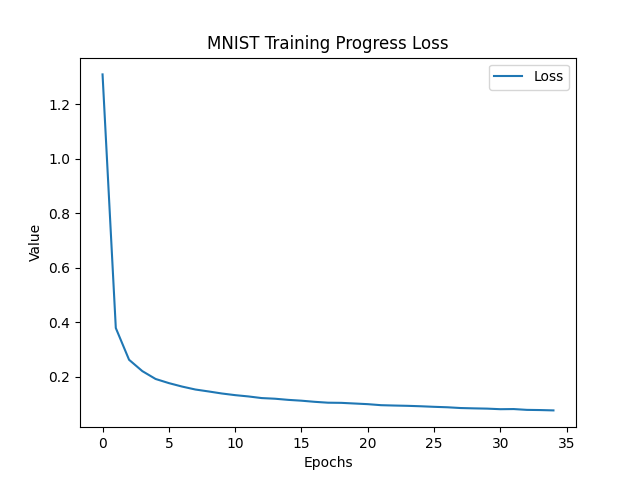
\includegraphics[width=0.95\textwidth]{gambar/best_plot_loss.png}
      \caption{\emph{Loss training} model}
      \label{fig:training-loss}
  	\end{figure}

	\begin{figure}[H]
      \centering
      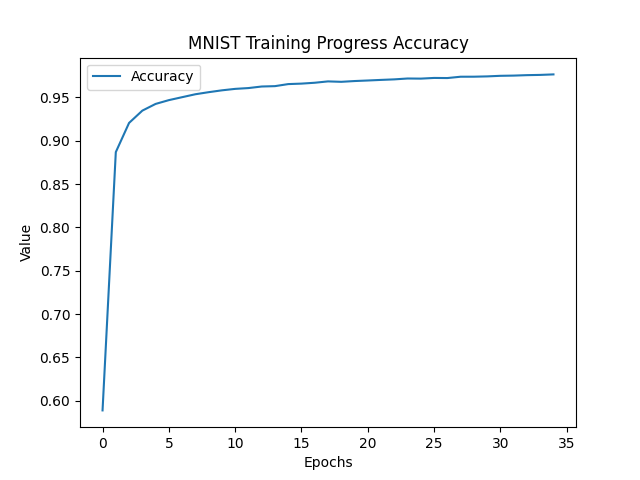
\includegraphics[width=0.95\textwidth]{gambar/best_plot_accuracy.png}
      \caption{\emph{Accuracy training} model}
      \label{fig:training-acc}
  	\end{figure}

	\begin{figure}[H]
      \centering
      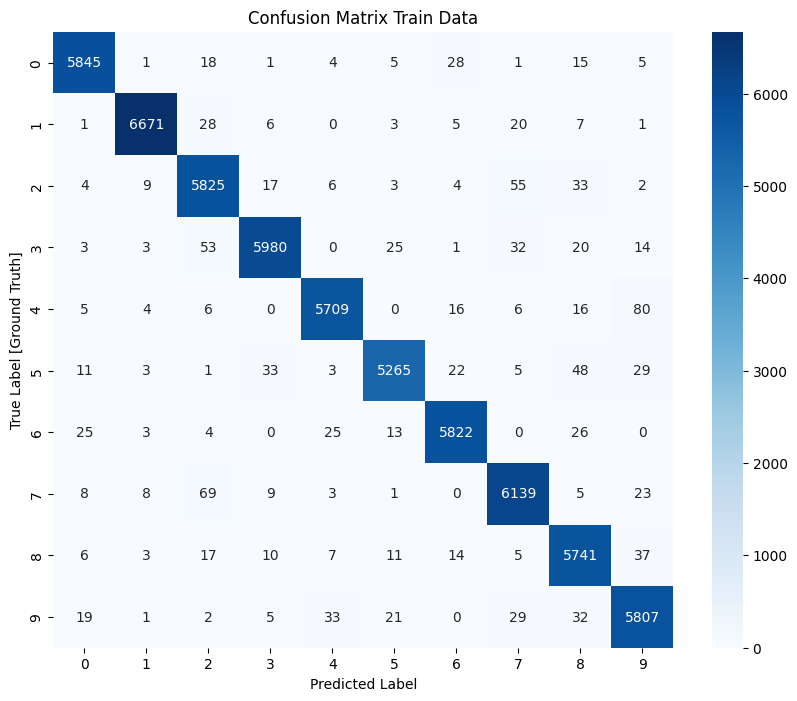
\includegraphics[width=0.95\textwidth]{gambar/confusion_matrix_train_model.png}
      \caption{\emph{Confusion Matrix Training} model}
      \label{fig:training-confussion-matrix}
  	\end{figure}

	\subsection{Kuantitasi Parameter Model CNN}
	....
	\begin{table}[htbp]
	\centering
		\caption{Parameter Model pada Python}
		\vspace{2mm}
		\small
		\begin{tabular}{llccc}
			\toprule
			\textbf{Parameter Name} & \textbf{Parameter Shape} & \textbf{Float Min} & \textbf{Float Max} & \textbf{Total Param} \\
			\midrule
			\textbf{conv1\_w} 		& (8, 1, 3, 3)  			& -0.41649 			& 0.22918 			& 72   \\
			\textbf{conv1\_b} 		& (8,)          			& -0.12903 			& 0.20184 			& 8    \\
			\textbf{conv2\_w} 		& (16, 8, 3, 3) 			& -0.4300774 		& 0.27402872 		& 1152 \\
			\textbf{conv2\_b} 		& (16,)         			& -0.14580758 		& 0.16609082 		& 16   \\
			\textbf{conv3\_w} 		& (32, 16, 3, 3)			& -0.27862 			& 0.29362 			& 4608 \\
			\textbf{conv3\_b} 		& (32,)         			& -0.11603 			& 0.10558 			& 32   \\
			\textbf{fc1\_w}   		& (16, 32)      			& -0.58693 			& 0.56456 			& 512  \\
			\textbf{fc1\_b}   		& (16,)         			& -0.00994 			& 0.01384 			& 16   \\
			\textbf{fc2\_w}   		& (10, 16)      			& -0.58495 			& 0.81792 			& 160  \\
			\textbf{fc2\_b}   		& (10,)         			& -0.07052 			& 0.13608 			& 10   \\
			\bottomrule
		\end{tabular}
	\end{table}

	\begin{table}[htbp]
	\centering
		\caption{Hasil Kuantisasi Parameter}
		\vspace{2mm}
		\small
		\begin{tabular}{lccccc}
			\toprule
			\textbf{Parameter Name} & \textbf{Mem Row (Lines)} & \textbf{Low Sat.} & \textbf{High Sat.} & \textbf{Quant Min} & \textbf{Quant Max} \\
			\midrule
			\textbf{conv1\_w} & 72   & 0 & 0 & -6824 & 3755  \\
			\textbf{conv1\_b} & 8    & 0 & 0 & -2114 & 3307  \\
			\textbf{conv2\_w} & 1152 & 0 & 0 & -7046 & 4490  \\
			\textbf{conv2\_b} & 16   & 0 & 0 & -2389 & 2721  \\
			\textbf{conv3\_w} & 4608 & 0 & 0 & -4565 & 4811  \\
			\textbf{conv3\_b} & 32   & 0 & 0 & -1901 & 1730  \\
			\textbf{fc1\_w}   & 512  & 0 & 0 & -9616 & 9250  \\
			\textbf{fc1\_b}   & 16   & 0 & 0 & -163  & 227   \\
			\textbf{fc2\_w}   & 160  & 0 & 0 & -9584 & 13401 \\
			\textbf{fc2\_b}   & 10   & 0 & 0 & -1155 & 2230  \\
			\bottomrule
		\end{tabular}
	\end{table}

\section{Hasil Implementasi CNN pada FPGA}
	\begin{figure}[H]
		\centering
		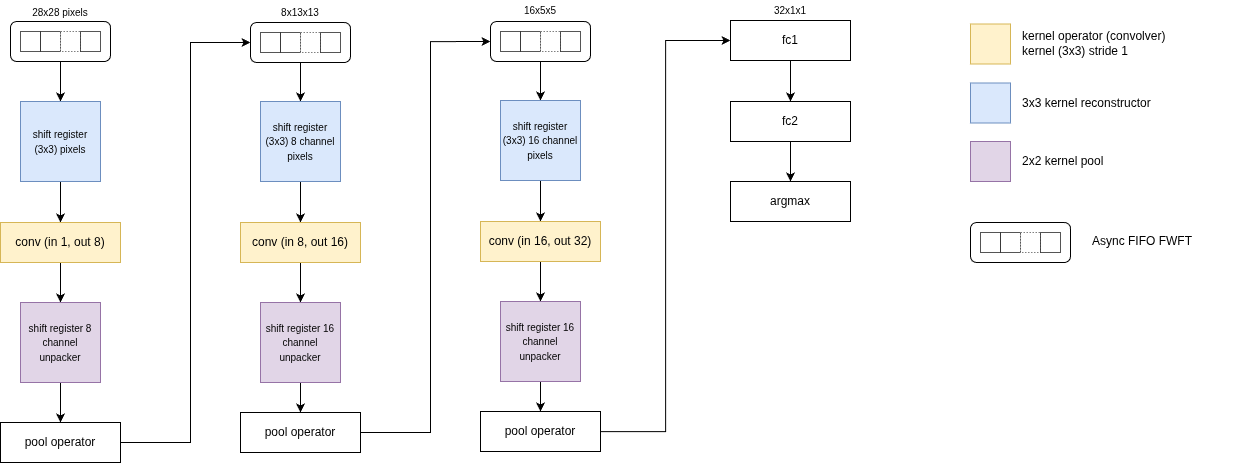
\includegraphics[width=0.95\textwidth]{gambar/cnn-accelerator-design.png}
		\caption{Desain CNN Accelerator pada FPGA}
		\label{fig:cnn-accelerator-design}
	\end{figure}
	\begin{table}[H]
		\centering
		\caption{Hasil \emph{Implement Running}}
		\label{implement-run-cnn}
		\begin{tabular}{|l|l|l|}
			\hline
			\textbf{Komponen} & \textbf{Resource Terpakai} & \textbf{Persentase} $\%$ \\
			\hline
			LUT & 13.742 & 22.11 \\
			Flip-Flop & 27.135 & 21.4 \\
			Block RAM & 18 & 13.33 \\
			DSP Slice & 232 DSP48E1 & 97.91 \\
			\hline
		\end{tabular}
	\end{table}
	\subsection{Hasil Latensi dan Throughput}
	....

\section{Hasil Uji Sanitasi Hardware}
	\subsection{Hasil Uji OV7670 pada \emph{Debug ILA}}
	....

	\subsection{Hasil Uji VGA PMOD Digilent}
	....
	
\begin{lstlisting}[language=Verilog, title={Kode Sanitasi VGA Verilog}, label={code:verilog-sanitize}]
case (h_count[9:7])
// White
3'd0: begin vga_r <= 4'hF;vga_g <= 4'hF;vga_b <= 4'hF;end
// Yellow
3'd1: begin vga_r <= 4'hF;vga_g <= 4'hF;vga_b <= 4'h0; end
// Cyan
3'd2: begin vga_r <= 4'h0;vga_g <= 4'hF;vga_b <= 4'hF; end
// Green
3'd3: begin vga_r <= 4'h0;vga_g <= 4'hF;vga_b <= 4'h0; end
// Magenta
3'd4: begin vga_r <= 4'hF;vga_g <= 4'h0;vga_b <= 4'hF; end
// Red
3'd5: begin vga_r <= 4'hF;vga_g <= 4'h0;vga_b <= 4'h0; end
// Blue
3'd6: begin vga_r <= 4'h0;vga_g <= 4'h0;vga_b <= 4'hF; end
// Black
default: begin vga_r  <= 4'h0;vga_g <= 4'h0;vga_b <= 4'h0; end
endcase
\end{lstlisting}

	\subsection{Hasil Uji Akses DDR3 SDRAM}
	....

\section{Hasil Integrasi Hardware}
	\subsection{Hasil Integrasi OV7670, VGA, dan DDR}
	\begin{table}[H]
      \centering
      \caption{Hasil \emph{Implement Running}}
      \label{implement-run-hardware}
      \begin{tabular}{|l|l|l|}
		  \hline
          \textbf{Komponen} & \textbf{Resource Terpakai} & \textbf{Persentase} $\%$ \\
          \hline
          LUT & 6.969 & 11 \\
          Flip-Flop & 6.357 & 5.01 \\
          Block RAM & 0.5 & 0.37 \\
          DSP Slice & 0 & 0.0 \\
          \hline
      \end{tabular}
  \end{table}
	....

	\subsection{Hasil Integrasi CNN Accelerator dengan OV7670, VGA, dan DDR}
	\begin{figure}[H]
		\centering
		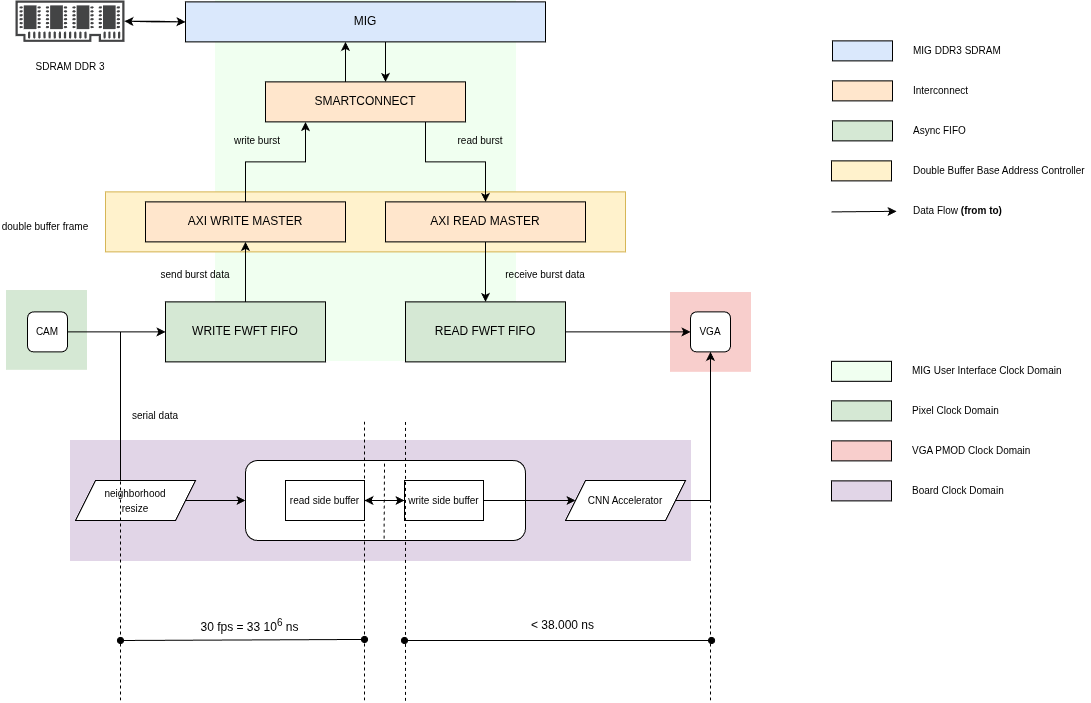
\includegraphics[width=0.95\textwidth]{gambar/full-sistem.png}
		\caption{Desian Akhir Integrasi}
		\label{fig:full-system-design}
	\end{figure}

	....

  	\begin{figure}[H]
		\centering
		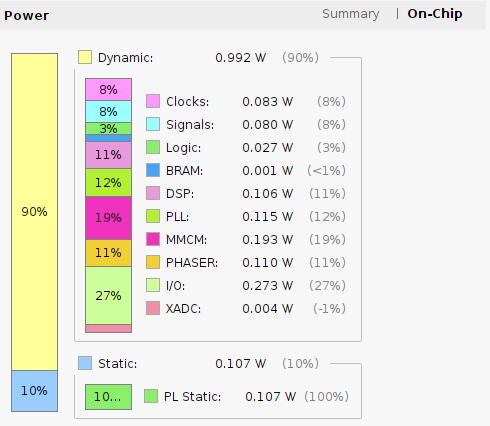
\includegraphics[width=0.95\textwidth]{gambar/power-analysis.png}
		\caption{Hasil Penggunaan Daya}
		\label{fig:full-system-design-power}
	\end{figure}

	\begin{table}[H]
		\centering
		\caption{Detail Hasil \emph{Implement Running}}
		\label{implement-run-fullimplementation}
		\begin{tabular}{|l|l|l|}
			\hline
			\textbf{Komponen} & \textbf{Resource Terpakai} & \textbf{Persentase} $\%$ \\
			\hline
			LUT & 20.755 & 32.74 \\
			Flip-Flop & 34.502 & 27.21 \\
			Block RAM & 19.5 & 14.44 \\
			DSP Slice & 235 DSP48E1 & 97.92 \\
			\hline
      	\end{tabular}
  	\end{table}

	\begin{table}[htbp]
	\centering
		\caption{Penggunaan Daya dan Temperature}
		\vspace{2mm}
		\small
		\begin{tabular}{llccc}
			\toprule
			\textbf{Total On Chip} 	& \textbf{Junction Temperature} & \textbf{Thermal Margin} 	& \textbf{Effective JA} \\
			\midrule
			\textbf{1.099 W} 		& \textbf{30.0 C}				& 55.0 C (11.9 W) 			& 4.6 C/W 				\\
			\bottomrule
		\end{tabular}
	\end{table}

	\begin{table}[htbp]
	\centering
		\caption{Hasil Routing Design}
		\vspace{2mm}
		\small
		\begin{tabular}{llccc}
			\toprule
			\textbf{Conflict Nets} 	& 
			\textbf{Unrouted Nets} & 
			\textbf{Partially Routed Nets} & 
			\textbf{Fully Routed Nets} \\
			\midrule
			0 & 
			0 & 
			0 & 
			63.141 \\
			\bottomrule
		\end{tabular}
	\end{table}

	\begin{table}[htbp]
	\centering
		\caption{Hasil \emph{Delayed} Design}
		\vspace{2mm}
		\small
		\begin{tabular}{llccc}
			\toprule
			\textbf{WNS} 	& 
			\textbf{TNS} & 
			\textbf{WHS} & 
			\textbf{WBSS} & 
			\textbf{TPWS} \\
			\midrule
			0.177 & 
			0.00 & 
			0.012 & 
			0.00 & 
			11.305 \\
			\bottomrule
		\end{tabular}
	\end{table}

\section{Hasil Evaluasi}
	\subsection{Hasil Evaluasi Model CNN}
	....
	\begin{figure}[H]
		\centering
		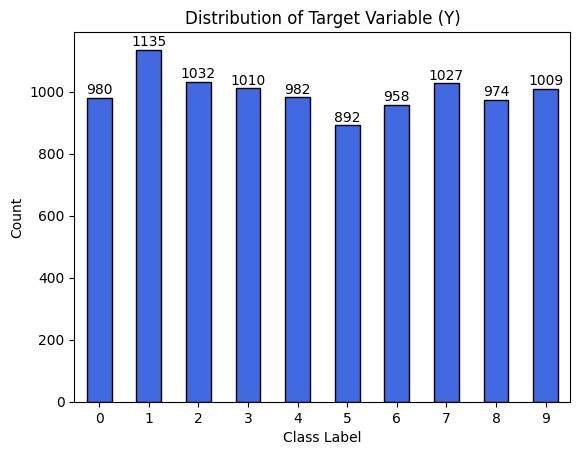
\includegraphics[width=0.95\textwidth]{gambar/data_test_distribution.png}
		\caption{Distribusi \emph{Test Dataset} yang digunakan}
		\label{fig:test-model-dataset}
	\end{figure}

	\begin{figure}[H]
      \centering
      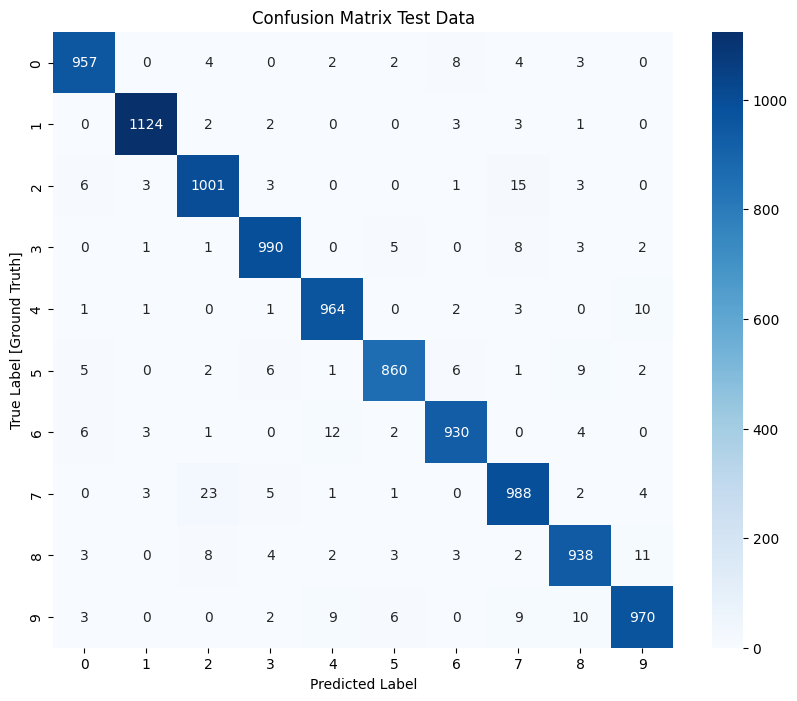
\includegraphics[width=0.95\textwidth]{gambar/confusion_matrix_test_model.png}
      \caption{\emph{Confusion Matrix testing} model}
      \label{fig:testing-confussion-matrix}
  	\end{figure}

	\subsection{Hasil Evaluasi Perbedaan Bit Model CNN}
	....
	\begin{figure}[H]
      \centering
      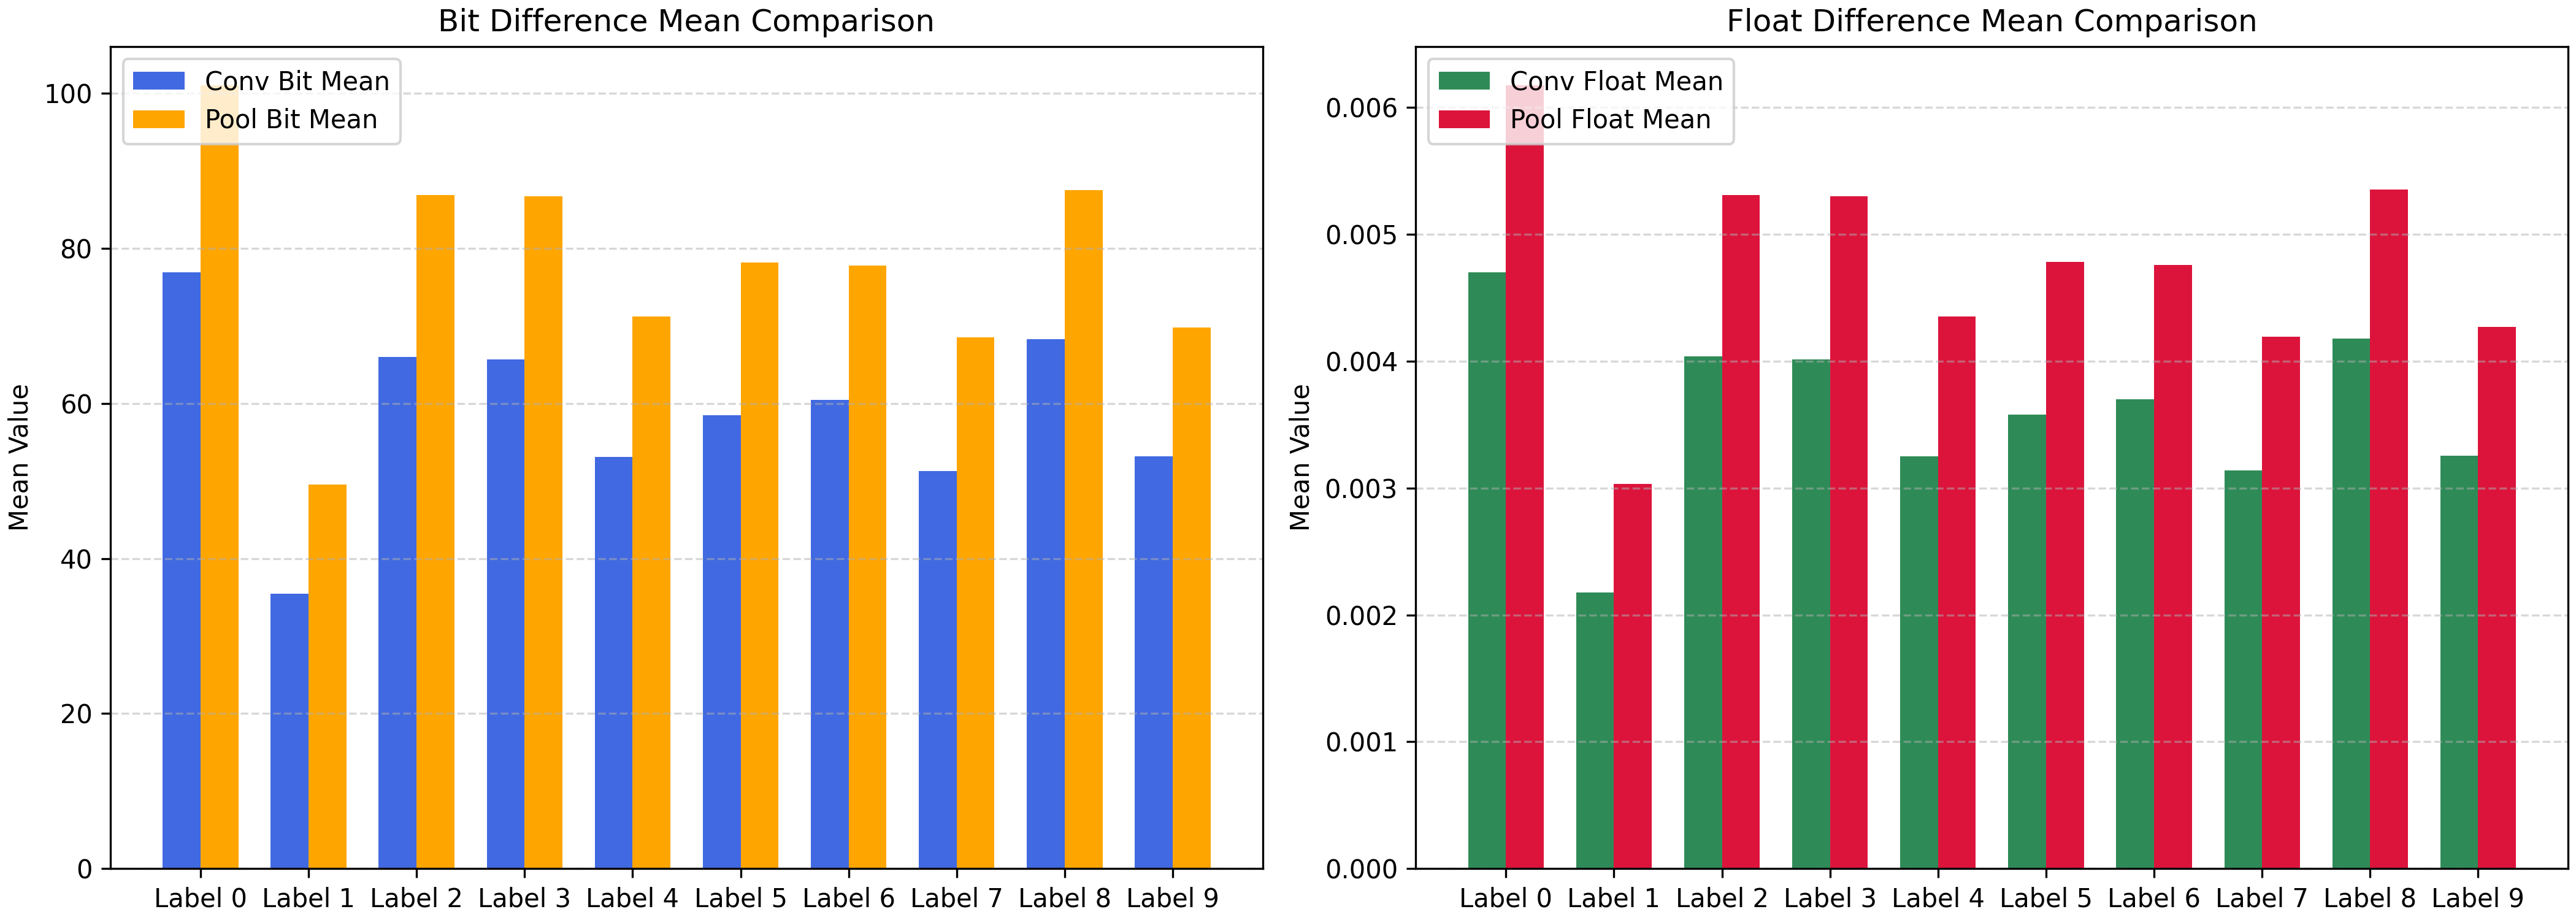
\includegraphics[width=0.95\textwidth]{gambar/train_results_all_labels_block1.png}
      \caption{Perbandingan \emph{Bit} dan \emph{Float value} pada \emph{Conv 1} dan \emph{Pool 1}}
      \label{fig:block1-bit-different}
  	\end{figure}

	\begin{figure}[H]
      \centering
      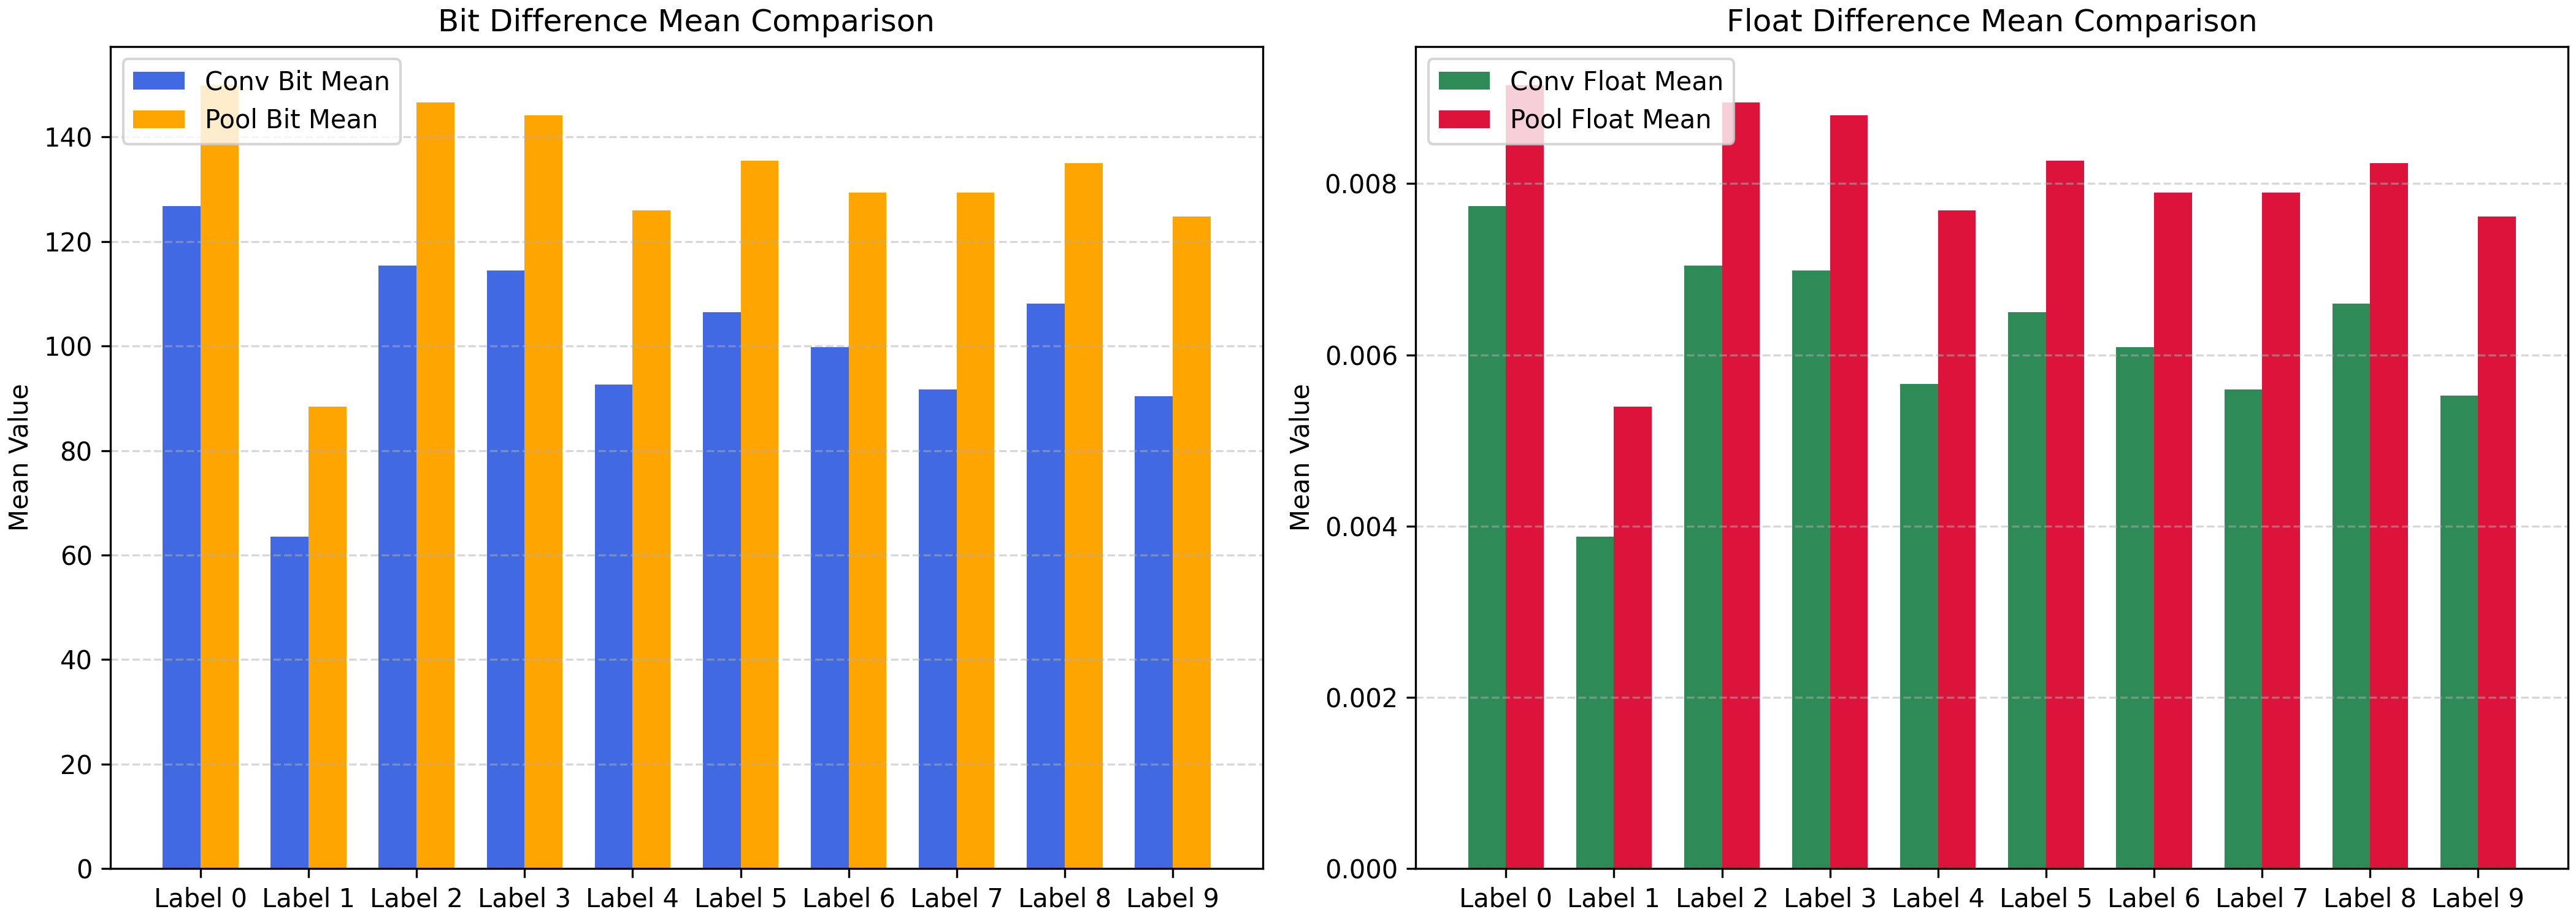
\includegraphics[width=0.95\textwidth]{gambar/train_results_all_labels_block2.png}
      \caption{Perbandingan \emph{Bit} dan \emph{Float value} pada \emph{Conv 2} dan \emph{Pool 2}}
      \label{fig:block2-bit-different}
  	\end{figure}

	\begin{figure}[H]
      \centering
      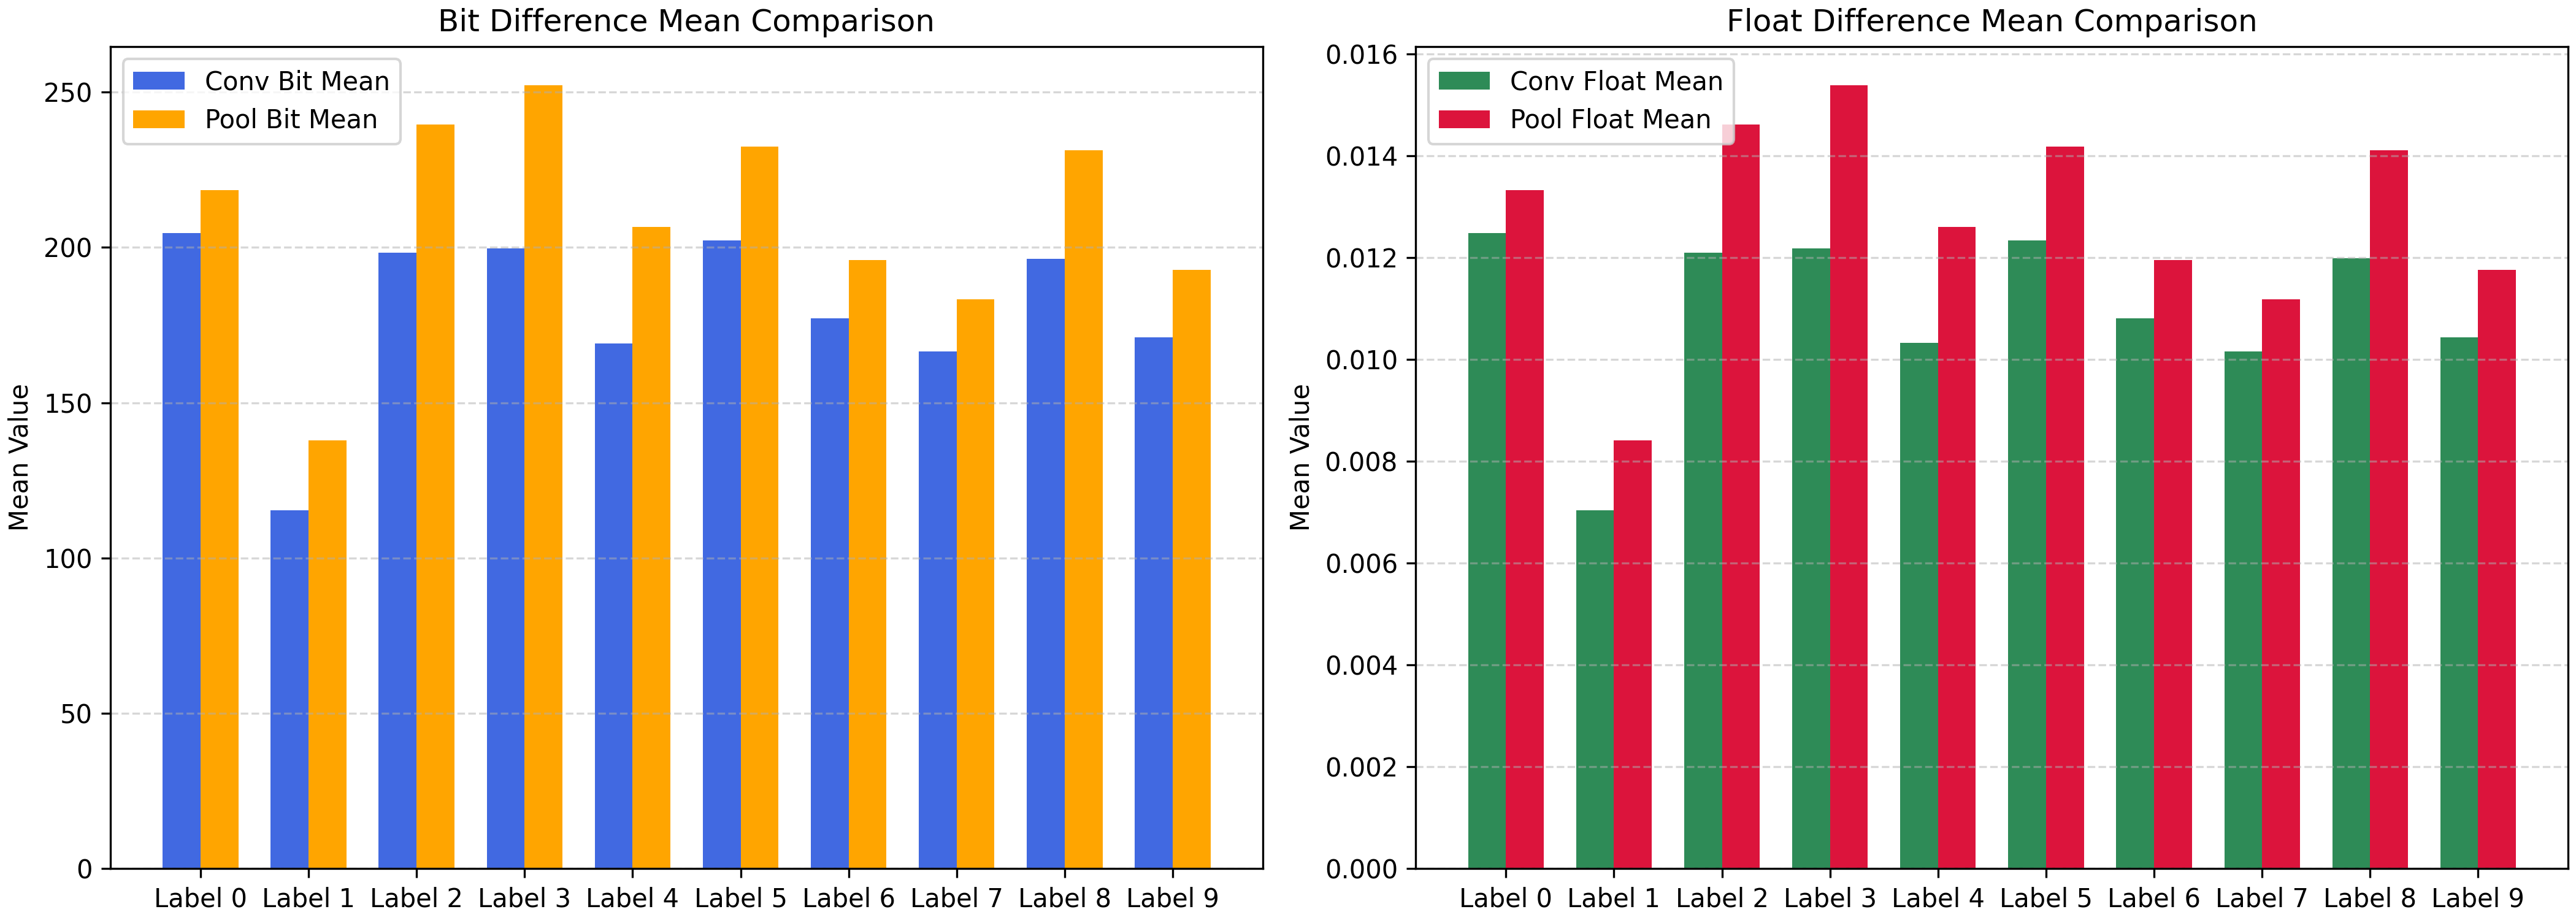
\includegraphics[width=0.95\textwidth]{gambar/train_results_all_labels_block3.png}
      \caption{Perbandingan \emph{Bit} dan \emph{Float value} pada \emph{Conv 3} dan \emph{Pool 3}}
      \label{fig:block3-bit-different}
  	\end{figure}

	\begin{figure}[H]
      \centering
      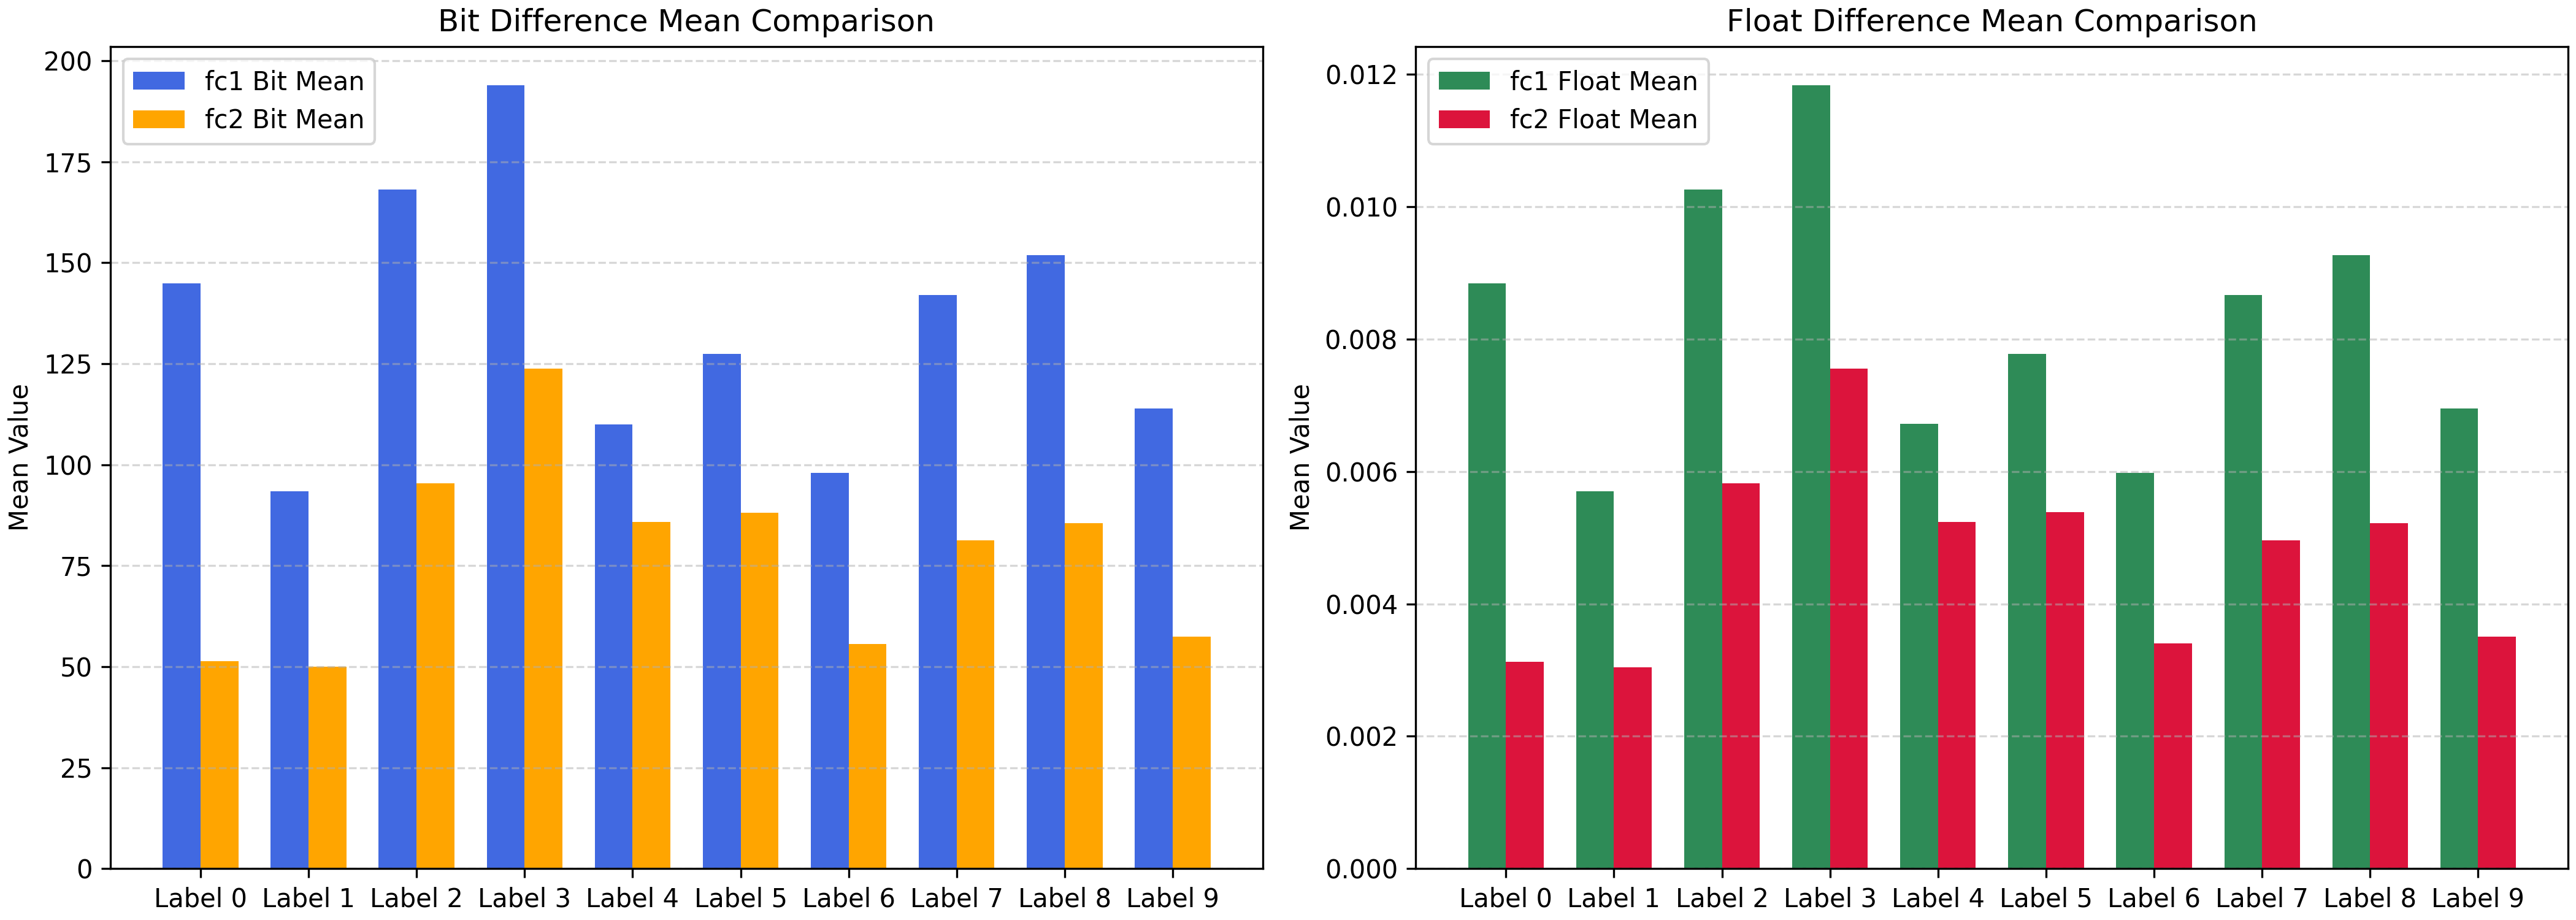
\includegraphics[width=0.95\textwidth]{gambar/train_results_all_labels_blockdense.png}
      \caption{Perbandingan \emph{Bit} dan \emph{Float value} pada \emph{Dense 1} dan \emph{Dense 2}}
      \label{fig:blockdense-bit-different}
  	\end{figure}

	\begin{figure}[H]
      \centering
      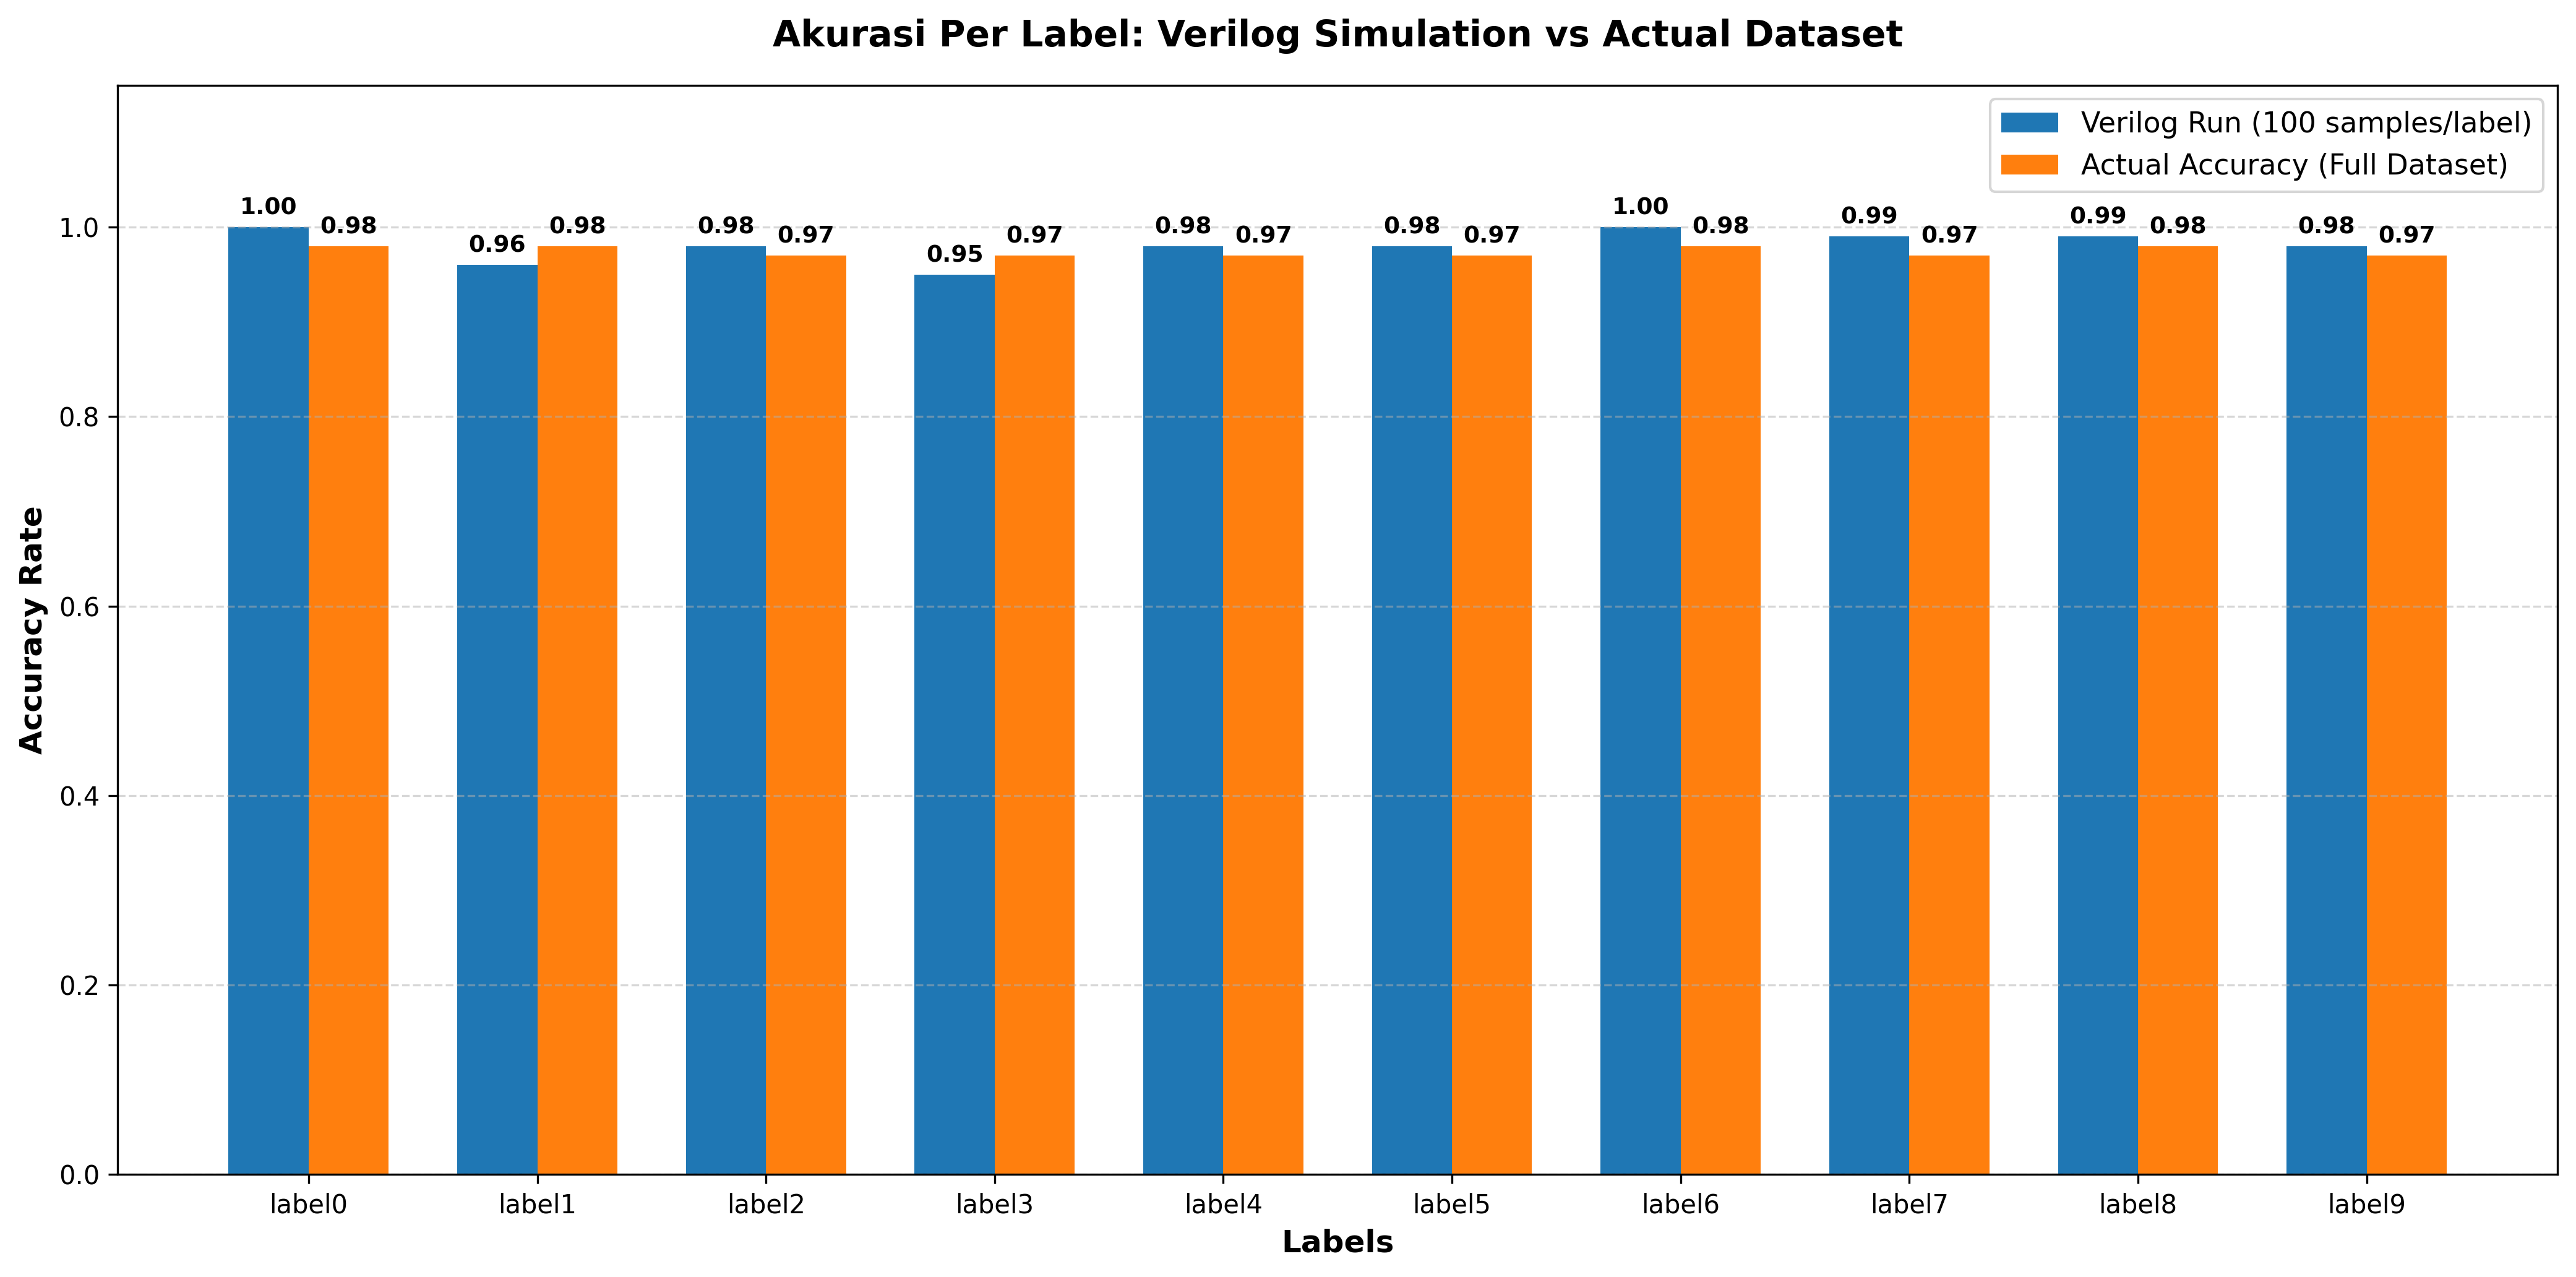
\includegraphics[width=0.95\textwidth]{gambar/train_accuracy-argmax.png}
      \caption{Perbedaan Akurasi}
      \label{fig:argmax-bit-accuracy}
  	\end{figure}

	\subsection{Hasil Evaluasi Inferensi Model di FPGA}
	....